 \documentclass{article}

% preambulo:
\usepackage[utf8]{inputenc}
% caracteres utf8 (tildes, enie) sin tener que usar comandos

\usepackage[spanish, es-tabla, es-nodecimaldot]{babel} 
% texto automatico en espaniol
% "tabla" en vez de "cuadro"
% no reemplaza puntos decimales por comas

%% NO AGREGAR PAQUETES ANTES DE ESTO, ES IMPORTANTE QUE BABEL ESTE PRIMERO

%%%%%%%%%%%%%%%%%%%%%%%%%%%%%%%%%
%% PAQUETES EXTRA %%%%%%%%%%%%%%%
%%%%%%%%%%%%%%%%%%%%%%%%%%%%%%%%%

\usepackage{subfiles}

%nuevo
\usepackage[notransparent]{svg}
%

\usepackage{amsmath} % PAQUETES DE MATEMATICA
\usepackage{amsfonts}
\usepackage{amssymb}

%puse esta cosa nueva---
\usepackage{csvsimple}

%-----
\usepackage{steinmetz} % comando \phase{}
\usepackage{units} % permite usar nicefrac
\usepackage{graphicx} % importar imagenes
\usepackage{float} % posicion H para floats
\usepackage[colorinlistoftodos]{todonotes}


\usepackage[a4paper, total={6in, 8in}]{geometry} 
% margenes correctos en subarchivos

\setlength{\parindent}{10pt}			%cuanta sangria al principio de un parrafo
\usepackage{indentfirst}				%pone sangria al primer parrafo de una seccion

\usepackage{listings}

\usepackage{color}

\definecolor{codegreen}{rgb}{0,0.6,0}
\definecolor{codegray}{rgb}{0.5,0.5,0.5}
\definecolor{codepurple}{rgb}{0.58,0,0.82}
\definecolor{backcolour}{rgb}{0.95,0.95,0.92}
 
\lstdefinestyle{mystyle}{
    backgroundcolor=\color{backcolour},   
    commentstyle=\color{codegreen},
    keywordstyle=\color{magenta},
    numberstyle=\tiny\color{codegray},
    stringstyle=\color{codepurple},
    basicstyle=\footnotesize,
    breakatwhitespace=false,         
    breaklines=true,                 
    captionpos=b,                    
    keepspaces=true,                 
    numbers=left,                    
    numbersep=5pt,                  
    showspaces=false,                
    showstringspaces=false,
    showtabs=false,                  
    tabsize=2
}
 
\lstset{style=mystyle}

%%%%%%%%%%%%%%%%%%%%%%%%%%%%%%%%%%%%%%%%%%%%%%%%%%%%%%%%%%%
%% NO AGREGAR PAQUETES DESPUES DE ESTO, ES IMPORTANTE QUE HYPERREF ESTE ULTIMO
\usepackage[hidelinks]{hyperref} % hipervinculos sin cajitas rojas
\usepackage{bm}


\usepackage{fancyhdr}

\geometry{top=2.5cm, bottom=2.0cm, left=2.25cm, right=2.25cm}

\lhead{Sistemas de Control 22.85}
\chead{TP4 - Control Carrito}
\rhead{ITBA}
\renewcommand{\headrulewidth}{1pt}
\renewcommand{\footrulewidth}{1pt}
\pagestyle{fancy}


\begin{document}

%\newgeometry{} % margenes default para la caratula
% caratula:
\begin{titlepage}
\newcommand{\HRule}{\rule{\linewidth}{0.5mm}}
\center
\mbox{\textsc{\LARGE \bfseries {Instituto Tecnol\'ogico de Buenos Aires}}}\\[1.5cm]
\textsc{\Large 22.85 - Sistemas de Control}\\[0.5cm]


\HRule \\[0.6cm]
{ \Huge \bfseries Trabajo de Laboratorio N$^{\circ}$4: Control de Carrito mediante controlador PID}\\[0.4cm] % Title of your document
\HRule \\[1.5cm]


{\large

\emph{Grupo 1}\\
\vspace{3px}

\begin{tabular}{lr} 	
\textsc{M\'aspero}, Martina  & 57120 \\
\textsc{Mestanza}, Joaqu\'in Mat\'ias  & 58288 \\
\textsc{Nowik}, Ariel Santiago  & 58309 \\
\textsc{Panaggio Venerandi}, Guido Martin  & 56214 \\
\textsc{Parra}, Roc\'io  & 57669 \\
\textsc{Regueira}, Marcelo Daniel  & 58300 \\

\end{tabular}

\vspace{20px}

\emph{Profesor}\\
\vspace{3px}
\textsc{Nasini}, V\'ictor Gustavo\\ 	
\vspace{100px}

\begin{tabular}{ll}

Presentado: & 27/11/2019\\

\end{tabular}

}

\vfill

\end{titlepage}


% indice:
\tableofcontents
\newpage

\section{PID: Introducción teórica}
Los controladores PID (proporcional, integrador y derivativo) proveen un control de lazo empleando feedback que es utilizado en la industria del control.
Un controlador PID calcula el error e(t) como la diferencia entre el setpoint(deseada) y una variable medida del proceso (la salida de la planta).


\begin{figure}[H]
\centering
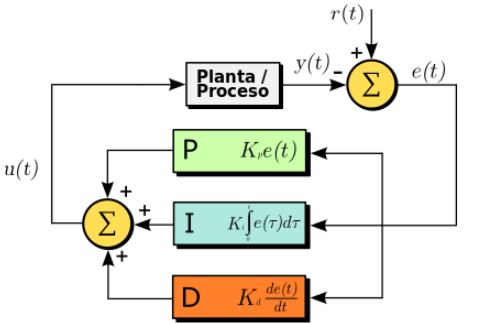
\includegraphics[width=0.5\linewidth]{images/PID.jpg}
\caption{Controlador PID: Esquema}
\label{fig:PID}
\end{figure}

Como se puede observar en la figura \ref{fig:PID} en los controladores PID se dispone de 3 constantes.
\begin{itemize}
  \item $K_p$: constante que acompaña al error 
  \item $K_i$: constante que acompaña a la integral del error 
  \item $K_d$: constante que acompaña a la derivada del error
  
\end{itemize}
\newpage
\section{Práctica}
Se ajustaron las constantes mediante el siguiente método:
\begin{itemize}
  \item Primero establecer $K_i=0$ y $K_d=0$. 
  \item Incrementar la $K_p$ hasta que la salida oscile
  \item Establecer $K_p$ a aproximadamente la mitad del valor configurado previamente
  \item Incrementar $K_i$ hasta que el proceso se ajuste en el tiempo requerido (precaución: subir mucho I puede causar inestabilidad)
  \item Finalmente, incrementar D si se necesita hasta que el lazo sea lo suficientemente rápido para alcanzar su referencia tras una variación brusca de la carga.
 
\newpage
\section{Resultados}
 
  
\end{itemize}
 

\end{document}
